\begin{figure}[h]
    \def\plotwidth{30}

    \newcommand{\nodesize}{22pt*1.4}
    \newcommand{\hsep}{56pt*1.4}
    \newcommand{\vsep}{28pt*1.4}

    \def\mriheight{5cm}

    \newcommand{\innerwidth}{0.2cm}
    \newcommand{\outerwidth}{0.6cm}
    \newcommand{\innerarrow}{{Latex[length=0.4cm, width=0.6cm]}}
    \newcommand{\outerarrow}{{Latex[length=0.8cm, width=1.4cm]}}

    \definecolor{outercolor}{RGB}{182, 182, 182}
    \colorlet{train-fill}{cb-green}

    \begin{tikzpicture}
        \newcommand{\mrivsep}{0.52}
        \newcommand{\mrihsep}{0.44}

        \node[anchor=north east] at (\plotwidth, 0) {};

        \newcommand{\mrilocation}[1]{($ (1, -2.2) + #1 $)}
        \newcommand{\modellocation}[1]{($ (0.5 * \plotwidth, -2.2) + #1 $)}
        \newcommand{\lrplocation}[1]{($ (0.5 * \plotwidth, -10.2) + #1 $)}

        \newcommand{\mrialpha}{0.2}
        \colorlet{predict-fill}{cb-blue}
        \colorlet{lrp-fill}{red}

        \node[inner sep=0pt, outer sep=0pt, label=\small{Structural MRI}] (input) at \mrilocation{(1 * \mrihsep, 0)} {
            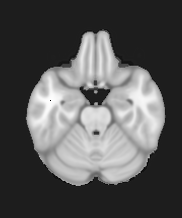
\includegraphics[height=\mriheight]{data/mris/slice_4.png}
        };

        \node[circle, inner sep=0pt, fill=none, outer sep=0pt, line width=0pt, draw=none] (n00) at \modellocation{(-3 * \hsep, 0)} {};

        \node[circle, minimum size=\nodesize, inner sep=0pt, fill=predict-fill!85, outer sep=0pt, line width=0pt, draw=predict-fill!85] (n10) at \modellocation{(-2 * \hsep, 2 * \vsep)} {};
        \node[circle, minimum size=\nodesize, inner sep=0pt, fill=predict-fill, outer sep=0pt, line width=0pt, draw=predict-fill] (n11) at \modellocation{(-2 * \hsep, 1 * \vsep)} {};
        \node[circle, minimum size=\nodesize, inner sep=0pt, fill=predict-fill!75, outer sep=0pt, line width=0pt, draw=predict-fill!75] (n12) at \modellocation{(-2 * \hsep, 0)} {};
        \node[circle, minimum size=\nodesize, inner sep=0pt, fill=predict-fill!15, outer sep=0pt, line width=0pt, draw=predict-fill!15] (n13) at \modellocation{(-2 * \hsep, -1 * \vsep)} {};
        \node[circle, minimum size=\nodesize, inner sep=0pt, fill=predict-fill!50, outer sep=0pt, line width=0pt, draw=predict-fill!50] (n14) at \modellocation{(-2 * \hsep, -2 * \vsep)} {};

        \node[circle, minimum size=\nodesize, inner sep=0pt, fill=predict-fill!15, outer sep=0pt, line width=0pt, draw=predict-fill!15] (n20) at \modellocation{(-1 * \hsep, 1.5 * \vsep)} {};
        \node[circle, minimum size=\nodesize, inner sep=0pt, fill=predict-fill!65, outer sep=0pt, line width=0pt, draw=predict-fill!65] (n21) at \modellocation{(-1 * \hsep, 0.5 * \vsep)} {};
        \node[circle, minimum size=\nodesize, inner sep=0pt, fill=predict-fill!90, outer sep=0pt, line width=0pt, draw=predict-fill!90] (n22) at \modellocation{(-1 * \hsep, -0.5 * \vsep)} {};
        \node[circle, minimum size=\nodesize, inner sep=0pt, fill=predict-fill!40, outer sep=0pt, line width=0pt, draw=predict-fill!40] (n23) at \modellocation{(-1 * \hsep, -1.5 * \vsep)} {};

        \node[circle, minimum size=\nodesize, inner sep=0pt, fill=predict-fill!80, outer sep=0pt, line width=0pt, draw=predict-fill!80] (n30) at \modellocation{(0 * \hsep, 1.5 * \vsep)} {};
        \node[circle, minimum size=\nodesize, inner sep=0pt, fill=predict-fill!55, outer sep=0pt, line width=0pt, draw=predict-fill!55] (n31) at \modellocation{(0 * \hsep, 0.5 * \vsep)} {};
        \node[circle, minimum size=\nodesize, inner sep=0pt, fill=predict-fill!15, outer sep=0pt, line width=0pt, draw=predict-fill!15] (n32) at \modellocation{(0 * \hsep, -0.5 * \vsep)} {};
        \node[circle, minimum size=\nodesize, inner sep=0pt, fill=predict-fill!75, outer sep=0pt, line width=0pt, draw=predict-fill!75] (n33) at \modellocation{(0 * \hsep, -1.5 * \vsep)} {};

        \node[circle, minimum size=\nodesize, inner sep=0pt, fill=predict-fill, outer sep=0pt, line width=0pt, draw=predict-fill] (n40) at \modellocation{(1 * \hsep, 1*\vsep)} {};
        \node[circle, minimum size=\nodesize, inner sep=0pt, fill=predict-fill!20, outer sep=0pt, line width=0pt, draw=predict-fill!20] (n41) at \modellocation{(1 * \hsep, 0*\vsep)} {};
        \node[circle, minimum size=\nodesize, inner sep=0pt, fill=predict-fill!15, outer sep=0pt, line width=0pt, draw=predict-fill!15] (n42) at \modellocation{(1 * \hsep, -1*\vsep)} {};

        \node[circle, minimum size=\nodesize, inner sep=0pt, fill=predict-fill!75, outer sep=0pt, line width=0pt, draw=predict-fill!75] (n50) at \modellocation{(2 * \hsep, 1*\vsep)} {};
        \node[circle, minimum size=\nodesize, inner sep=0pt, fill=predict-fill!35, outer sep=0pt, line width=0pt, draw=predict-fill!35] (n51) at \modellocation{(2 * \hsep, 0*\vsep)} {};
        \node[circle, minimum size=\nodesize, inner sep=0pt, fill=predict-fill!65, outer sep=0pt, line width=0pt, draw=predict-fill!65] (n52) at \modellocation{(2 * \hsep, -1*\vsep)} {};

        \node[circle, minimum size=\nodesize, inner sep=0pt, fill=predict-fill!85, outer sep=0pt, line width=0pt, draw=predict-fill!85] (output) at \modellocation{(3 * \hsep, 0)} {};

        \node[anchor=west, font=\small\linespread{0.8}\selectfont, align=center] (diagnosis) at \modellocation{(4.5 * \hsep, 0)} {Predicted probability\\of dementia};

        \draw[
            color=predict-fill!85,
            -\innerarrow,
            line width=\innerwidth
        ] (n00) to [out=20,in=200] (n10) {};
        \draw[
            color=predict-fill,
            -\innerarrow,
            line width=\innerwidth
        ] (n00) to [out=10,in=190] (n11) {};
        \draw[
            color=predict-fill!75,
            -\innerarrow,
            line width=\innerwidth
        ] (n00) to [out=0,in=180] (n12) {};
        \draw[
            color=predict-fill!15,
            -\innerarrow,
            line width=\innerwidth
        ] (n00) to [out=-10,in=170] (n13) {};
        \draw[
            color=predict-fill!50,
            -\innerarrow,
            line width=\innerwidth
        ] (n00) to [out=-20,in=160] (n14) {};

        \draw[
            color=predict-fill!75,
            -\innerarrow,
            line width=\innerwidth
        ] (n10) to [out=-5,in=175] (n20) {};
        \draw[
            color=predict-fill!50,
            -\innerarrow,
            line width=\innerwidth
        ] (n10) to [out=-15,in=165] (n21) {};
        \draw[
            color=predict-fill!55,
            -\innerarrow,
            line width=\innerwidth
        ] (n10) to [out=-25,in=155] (n22) {};
        \draw[
            color=predict-fill!85,
            -\innerarrow,
            line width=\innerwidth
        ] (n10) to [out=-35,in=145] (n23) {};

        \draw[
            color=predict-fill!45,
            -\innerarrow,
            line width=\innerwidth
        ] (n11) to [out=5,in=185] (n20) {};
        \draw[
            color=predict-fill!50,
            -\innerarrow,
            line width=\innerwidth
        ] (n11) to [out=-5,in=175] (n21) {};
        \draw[
            color=predict-fill,
            -\innerarrow,
            line width=\innerwidth
        ] (n11) to [out=-15,in=165] (n22) {};
        \draw[
            color=predict-fill!15,
            -\innerarrow,
            line width=\innerwidth
        ] (n11) to [out=-25,in=155] (n23) {};

        \draw[
            color=predict-fill!35,
            -\innerarrow,
            line width=\innerwidth
        ] (n12) to [out=15,in=195] (n20) {};
        \draw[
            color=predict-fill!90,
            -\innerarrow,
            line width=\innerwidth
        ] (n12) to [out=5,in=185] (n21) {};
        \draw[
            color=predict-fill!80,
            -\innerarrow,
            line width=\innerwidth
        ] (n12) to [out=-5,in=175] (n22) {};
        \draw[
            color=predict-fill!20,
            -\innerarrow,
            line width=\innerwidth
        ] (n12) to [out=-15,in=165] (n23) {};

        \draw[
            color=predict-fill!55,
            -\innerarrow,
            line width=\innerwidth
        ] (n13) to [out=25,in=205] (n20) {};
        \draw[
            color=predict-fill!65,
            -\innerarrow,
            line width=\innerwidth
        ] (n13) to [out=15,in=195] (n21) {};
        \draw[
            color=predict-fill!35,
            -\innerarrow,
            line width=\innerwidth
        ] (n13) to [out=5,in=185] (n22) {};
        \draw[
            color=predict-fill!45,
            -\innerarrow,
            line width=\innerwidth
        ] (n13) to [out=-5,in=175] (n23) {};

        \draw[
            color=predict-fill!10,
            -\innerarrow,
            line width=\innerwidth
        ] (n14) to [out=35,in=215] (n20) {};
        \draw[
            color=predict-fill!90,
            -\innerarrow,
            line width=\innerwidth
        ] (n14) to [out=25,in=205] (n21) {};
        \draw[
            color=predict-fill!80,
            -\innerarrow,
            line width=\innerwidth
        ] (n14) to [out=15,in=195] (n22) {};
        \draw[
            color=predict-fill!35,
            -\innerarrow,
            line width=\innerwidth
        ] (n14) to [out=5,in=185] (n23) {};

        \draw[
            color=predict-fill!75,
            -\innerarrow,
            line width=\innerwidth
        ] (n20) to [out=0,in=180] (n30) {};
        \draw[
            color=predict-fill!50,
            -\innerarrow,
            line width=\innerwidth
        ] (n20) to [out=-10,in=170] (n31) {};
        \draw[
            color=predict-fill!85,
            -\innerarrow,
            line width=\innerwidth
        ] (n20) to [out=-20,in=160] (n32) {};
        \draw[
            color=predict-fill!45,
            -\innerarrow,
            line width=\innerwidth
        ] (n20) to [out=-30,in=150] (n33) {};

        \draw[
            color=predict-fill!20,
            -\innerarrow,
            line width=\innerwidth
        ] (n21) to [out=10,in=190] (n30) {};
        \draw[
            color=predict-fill!35,
            -\innerarrow,
            line width=\innerwidth
        ] (n21) to [out=0,in=180] (n31) {};
        \draw[
            color=predict-fill!15,
            -\innerarrow,
            line width=\innerwidth
        ] (n21) to [out=-10,in=170] (n32) {};
        \draw[
            color=predict-fill!90,
            -\innerarrow,
            line width=\innerwidth
        ] (n21) to [out=-20,in=160] (n33) {};

        \draw[
            color=predict-fill!65,
            -\innerarrow,
            line width=\innerwidth
        ] (n22) to [out=20,in=200] (n30) {};
        \draw[
            color=predict-fill!20,
            -\innerarrow,
            line width=\innerwidth
        ] (n22) to [out=10,in=190] (n31) {};
        \draw[
            color=predict-fill!30,
            -\innerarrow,
            line width=\innerwidth
        ] (n22) to [out=0,in=180] (n32) {};
        \draw[
            color=predict-fill!40,
            -\innerarrow,
            line width=\innerwidth
        ] (n22) to [out=-10,in=170] (n33) {};

        \draw[
            color=predict-fill,
            -\innerarrow,
            line width=\innerwidth
        ] (n23) to [out=30,in=210] (n30) {};
        \draw[
            color=predict-fill!15,
            -\innerarrow,
            line width=\innerwidth
        ] (n23) to [out=20,in=200] (n31) {};
        \draw[
            color=predict-fill!75,
            -\innerarrow,
            line width=\innerwidth
        ] (n23) to [out=10,in=190] (n32) {};
        \draw[
            color=predict-fill!35,
            -\innerarrow,
            line width=\innerwidth
        ] (n23) to [out=0,in=180] (n33) {};

        \draw[
            color=predict-fill!70,
            -\innerarrow,
            line width=\innerwidth
        ] (n30) to [out=-5,in=175] (n40) {};
        \draw[
            color=predict-fill!80,
            -\innerarrow,
            line width=\innerwidth
        ] (n30) to [out=-15,in=165] (n41) {};
        \draw[
            color=predict-fill!20,
            -\innerarrow,
            line width=\innerwidth
        ] (n30) to [out=-25,in=155] (n42) {};

        \draw[
            color=predict-fill!60,
            -\innerarrow,
            line width=\innerwidth
        ] (n31) to [out=5,in=185] (n40) {};
        \draw[
            color=predict-fill!95,
            -\innerarrow,
            line width=\innerwidth
        ] (n31) to [out=-5,in=175] (n41) {};
        \draw[
            color=predict-fill!35,
            -\innerarrow,
            line width=\innerwidth
        ] (n31) to [out=-15,in=165] (n42) {};

        \draw[
            color=predict-fill!75,
            -\innerarrow,
            line width=\innerwidth
        ] (n32) to [out=15,in=195] (n40) {};
        \draw[
            color=predict-fill!20,
            -\innerarrow,
            line width=\innerwidth
        ] (n32) to [out=5,in=185] (n41) {};
        \draw[
            color=predict-fill!15,
            -\innerarrow,
            line width=\innerwidth
        ] (n32) to [out=-5,in=175] (n42) {};

        \draw[
            color=predict-fill!40,
            -\innerarrow,
            line width=\innerwidth
        ] (n33) to [out=25,in=205] (n40) {};
        \draw[
            color=predict-fill!80,
            -\innerarrow,
            line width=\innerwidth
        ] (n33) to [out=15,in=195] (n41) {};
        \draw[
            color=predict-fill!50,
            -\innerarrow,
            line width=\innerwidth
        ] (n33) to [out=5,in=185] (n42) {};

        \draw[
            color=predict-fill!25,
            -\innerarrow,
            line width=\innerwidth
        ] (n40) to [out=0,in=180] (n50) {};
        \draw[
            color=predict-fill!50,
            -\innerarrow,
            line width=\innerwidth
        ] (n40) to [out=-10,in=170] (n51) {};
        \draw[
            color=predict-fill!45,
            -\innerarrow,
            line width=\innerwidth
        ] (n40) to [out=-20,in=160] (n52) {};

        \draw[
            color=predict-fill!90,
            -\innerarrow,
            line width=\innerwidth
        ] (n41) to [out=10,in=190] (n50) {};
        \draw[
            color=predict-fill!10,
            -\innerarrow,
            line width=\innerwidth
        ] (n41) to [out=0,in=180] (n51) {};
        \draw[
            color=predict-fill!75,
            -\innerarrow,
            line width=\innerwidth
        ] (n41) to [out=-10,in=170] (n52) {};

        \draw[
            color=predict-fill!60,
            -\innerarrow,
            line width=\innerwidth
        ] (n42) to [out=20,in=200] (n50) {};
        \draw[
            color=predict-fill!25,
            -\innerarrow,
            line width=\innerwidth
        ] (n42) to [out=10,in=190] (n51) {};
        \draw[
            color=predict-fill!15,
            -\innerarrow,
            line width=\innerwidth
        ] (n42) to [out=0,in=180] (n52) {};

        \draw[
            color=predict-fill!95,
            -\innerarrow,
            line width=\innerwidth
        ] (n50) to [out=-10,in=170] (output) {};
        \draw[
            color=predict-fill!25,
            -\innerarrow,
            line width=\innerwidth
        ] (n51) to [out=0,in=180] (output) {};
        \draw[
            color=predict-fill!50,
            -\innerarrow,
            line width=\innerwidth
        ] (n52) to [out=10,in=190] (output) {};

        \draw[black] (n00.center) --
                        ($ (n00) + (0, 2*\vsep+0.5*\nodesize+2pt) $) --
                        ($ (n00) + (6*\hsep+0.5*\nodesize+2pt, 2*\vsep+0.5*\nodesize+2pt) $) --
                        ($ (n00) + (6*\hsep+0.5*\nodesize+2pt, -2*\vsep-0.5*\nodesize-2pt) $) --
                        ($ (n00) + (0, -2*\vsep-0.5*\nodesize-2pt) $) -- (n00.center);

        \node[] at ($ (n30) + (0, \vsep+0.5*\nodesize) $) {Simple Fully Convolutional Network};

        \draw[
            color=outercolor,
            -\outerarrow,
            line width=\outerwidth
        ] (input) to [out=0,in=180] (n00) {};
        \draw[
            color=outercolor,
            -\outerarrow,
            line width=\outerwidth
        ] (output) to [out=0,in=180] (diagnosis) {};

        \node[circle, inner sep=0pt, fill=none, outer sep=0pt, line width=0pt, draw=none] (n00) at \lrplocation{(-3 * \hsep, 0)} {};

        \node[circle, minimum size=\nodesize, inner sep=0pt, fill={rgb:black,5;orange,1}, outer sep=0pt, line width=0pt, draw={rgb:black,5;orange,1}] (n10) at \lrplocation{(-2 * \hsep, 2 * \vsep)} {};
        \node[circle, minimum size=\nodesize, inner sep=0pt, fill={rgb:black,3;red,1}, outer sep=0pt, line width=0pt, draw={rgb:black,3;red,1}] (n11) at \lrplocation{(-2 * \hsep, 1 * \vsep)} {};
        \node[circle, minimum size=\nodesize, inner sep=0pt, fill=yellow, outer sep=0pt, line width=0pt, draw=yellow] (n12) at \lrplocation{(-2 * \hsep, 0)} {};
        \node[circle, minimum size=\nodesize, inner sep=0pt, fill=black, outer sep=0pt, line width=0pt, draw=black] (n13) at \lrplocation{(-2 * \hsep, -1 * \vsep)} {};
        \node[circle, minimum size=\nodesize, inner sep=0pt, fill=red, outer sep=0pt, line width=0pt, draw=red] (n14) at \lrplocation{(-2 * \hsep, -2 * \vsep)} {};

        \node[circle, minimum size=\nodesize, inner sep=0pt, fill={rgb:black,5;white,2;orange,1}, outer sep=0pt, line width=0pt, draw={rgb:black,5;white,2;orange,1}] (n20) at \lrplocation{(-1 * \hsep, 1.5 * \vsep)} {};
        \node[circle, minimum size=\nodesize, inner sep=0pt, fill={rgb:red,10;yellow,6}, outer sep=0pt, line width=0pt, draw={rgb:red,10;yellow,4}] (n21) at \lrplocation{(-1 * \hsep, 0.5 * \vsep)} {};
        \node[circle, minimum size=\nodesize, inner sep=0pt, fill={rgb:red,10;yellow,1}, outer sep=0pt, line width=0pt, draw={rgb:red,10;yellow,1}] (n22) at \lrplocation{(-1 * \hsep, -0.5 * \vsep)} {};
        \node[circle, minimum size=\nodesize, inner sep=0pt, fill={rgb:black,10;red,2}, outer sep=0pt, line width=0pt, draw={rgb:black,10;red,2}] (n23) at \lrplocation{(-1 * \hsep, -1.5 * \vsep)} {};

        \node[circle, minimum size=\nodesize, inner sep=0pt, fill={rgb:red,3;orange,2}, outer sep=0pt, line width=0pt, draw={rgb:red,3;orange,1}] (n30) at \lrplocation{(0 * \hsep, 1.5 * \vsep)} {};
        \node[circle, minimum size=\nodesize, inner sep=0pt, fill={rgb:yellow,3;orange,1}, outer sep=0pt, line width=0pt, draw={rgb:yellow,3;orange,1}] (n31) at \lrplocation{(0 * \hsep, 0.5 * \vsep)} {};
        \node[circle, minimum size=\nodesize, inner sep=0pt, fill={rgb:black,10;white,5;red,1}, outer sep=0pt, line width=0pt, draw={rgb:black,10;white,5;red,1}] (n32) at \lrplocation{(0 * \hsep, -0.5 * \vsep)} {};
        \node[circle, minimum size=\nodesize, inner sep=0pt, fill={rgb:gray,5;red,1}, outer sep=0pt, line width=0pt, draw={rgb:gray,5;red,1}] (n33) at \lrplocation{(0 * \hsep, -1.5 * \vsep)} {};

        \node[circle, minimum size=\nodesize, inner sep=0pt, fill={rgb:yellow,10;orange,1}, outer sep=0pt, line width=0pt, draw={rgb:yellow,10;orange,1}] (n40) at \lrplocation{(1 * \hsep, 1*\vsep)} {};
        \node[circle, minimum size=\nodesize, inner sep=0pt, fill={rgb:red,1}, outer sep=0pt, line width=0pt, draw={rgb:red,1}] (n41) at \lrplocation{(1 * \hsep, 0*\vsep)} {};
        \node[circle, minimum size=\nodesize, inner sep=0pt, fill={rgb:black,10;white,15;red,2}, outer sep=0pt, line width=0pt, draw={rgb:black,10;white,15;red,2}] (n42) at \lrplocation{(1 * \hsep, -1*\vsep)} {};

        \node[circle, minimum size=\nodesize, inner sep=0pt, fill={rgb:red,5;black,1;yellow,2}, outer sep=0pt, line width=0pt, draw={rgb:red,5;black,1;yellow,2}] (n50) at \lrplocation{(2 * \hsep, 1*\vsep)} {};
        \node[circle, minimum size=\nodesize, inner sep=0pt, fill={rgb:gray,5;red,1}, outer sep=0pt, line width=0pt, draw={rgb:gray,5;red,1}] (n51) at \lrplocation{(2 * \hsep, 0*\vsep)} {};
        \node[circle, minimum size=\nodesize, inner sep=0pt, fill={rgb:yellow,5;orange,1}, outer sep=0pt, line width=0pt, draw={rgb:yellow,5;orange,1}] (n52) at \lrplocation{(2 * \hsep, -1*\vsep)} {};

        \node[circle, minimum size=\nodesize, inner sep=0pt, fill={rgb:orange,7;yellow,4;black,1}, outer sep=0pt, line width=0pt, draw={rgb:orange,7;yellow,4;black,1}] (n60) at \lrplocation{(3 * \hsep, 0)} {};

        \draw[
            color={rgb:black,5;orange,1},
            \innerarrow-,
            line width=\innerwidth
        ] (n00) to [out=20,in=200] (n10) {};
        \draw[
            color={rgb:black,3;red,1},
            \innerarrow-,
            line width=\innerwidth
        ] (n00) to [out=10,in=190] (n11) {};
        \draw[
            color=yellow,
            \innerarrow-,
            line width=\innerwidth
        ] (n00) to [out=0,in=180] (n12) {};
        \draw[
            color=black,
            \innerarrow-,
            line width=\innerwidth
        ] (n00) to [out=-10,in=170] (n13) {};
        \draw[
            color=red,
            \innerarrow-,
            line width=\innerwidth
        ] (n00) to [out=-20,in=160] (n14) {};

        \draw[
            color={rgb:black,5;white,1;orange,1},
            \innerarrow-,
            line width=\innerwidth
        ] (n10) to [out=-5,in=175] (n20) {};
        \draw[
            color={rgb:black,3;orange,1},
            \innerarrow-,
            line width=\innerwidth
        ] (n10) to [out=-15,in=165] (n21) {};
        \draw[
            color={rgb:black,4;red,2;yellow,1},
            \innerarrow-,
            line width=\innerwidth
        ] (n10) to [out=-25,in=155] (n22) {};
        \draw[
            color={rgb:black,3;red,1},
            \innerarrow-,
            line width=\innerwidth
        ] (n10) to [out=-35,in=145] (n23) {};

        \draw[
            color={rgb:black,10;orange,2},
            \innerarrow-,
            line width=\innerwidth
        ] (n11) to [out=5,in=185] (n20) {};
        \draw[
            color={rgb:black,3;orange,1},
            \innerarrow-,
            line width=\innerwidth
        ] (n11) to [out=-5,in=175] (n21) {};
        \draw[
            color={rgb:black,3;red,1},
            \innerarrow-,
            line width=\innerwidth
        ] (n11) to [out=-15,in=165] (n22) {};
        \draw[
            color={rgb:black,10;red,1},
            \innerarrow-,
            line width=\innerwidth
        ] (n11) to [out=-25,in=155] (n23) {};

        \draw[
            color={rgb:black,5;orange,3},
            \innerarrow-,
            line width=\innerwidth
        ] (n12) to [out=15,in=195] (n20) {};
        \draw[
            color={rgb:red,3;yellow,5},
            \innerarrow-,
            line width=\innerwidth
        ] (n12) to [out=5,in=185] (n21) {};
        \draw[
            color={rgb:red,5;yellow,3},
            \innerarrow-,
            line width=\innerwidth
        ] (n12) to [out=-5,in=175] (n22) {};
        \draw[
            color={rgb:black,5;orange,2},
            \innerarrow-,
            line width=\innerwidth
        ] (n12) to [out=-15,in=165] (n23) {};

        \draw[
            color={rgb:black,5;red,1},
            \innerarrow-,
            line width=\innerwidth
        ] (n13) to [out=25,in=205] (n20) {};
        \draw[
            color={rgb:black,5;orange,2},
            \innerarrow-,
            line width=\innerwidth
        ] (n13) to [out=15,in=195] (n21) {};
        \draw[
            color={rgb:black,5;red,3},
            \innerarrow-,
            line width=\innerwidth
        ] (n13) to [out=5,in=185] (n22) {};
        \draw[
            color=black,
            \innerarrow-,
            line width=\innerwidth
        ] (n13) to [out=-5,in=175] (n23) {};

        \draw[
            color={rgb:black,5;orange,2},
            \innerarrow-,
            line width=\innerwidth
        ] (n14) to [out=35,in=215] (n20) {};
        \draw[
            color={rgb:red,3;orange,1},
            \innerarrow-,
            line width=\innerwidth
        ] (n14) to [out=25,in=205] (n21) {};
        \draw[
            color={rgb:red,5;yellow,2},
            \innerarrow-,
            line width=\innerwidth
        ] (n14) to [out=15,in=195] (n22) {};
        \draw[
            color={rgb:black,5;red,3},
            \innerarrow-,
            line width=\innerwidth
        ] (n14) to [out=5,in=185] (n23) {};

        \draw[
            color={rgb:black,1;red,1},
            \innerarrow-,
            line width=\innerwidth
        ] (n20) to [out=0,in=180] (n30) {};
        \draw[
            color={rgb:black,3;orange,1},
            \innerarrow-,
            line width=\innerwidth
        ] (n20) to [out=-10,in=170] (n31) {};
        \draw[
            color={rgb:black,10;red,1},
            \innerarrow-,
            line width=\innerwidth
        ] (n20) to [out=-20,in=160] (n32) {};
        \draw[
            color={rgb:black,5;red,1},
            \innerarrow-,
            line width=\innerwidth
        ] (n20) to [out=-30,in=150] (n33) {};

        \draw[
            color={rgb:orange,5;red,2},
            \innerarrow-,
            line width=\innerwidth
        ] (n21) to [out=10,in=190] (n30) {};
        \draw[
            color={rgb:yellow,10;orange,4},
            \innerarrow-,
            line width=\innerwidth
        ] (n21) to [out=0,in=180] (n31) {};
        \draw[
            color={rgb:black,2;red,1},
            \innerarrow-,
            line width=\innerwidth
        ] (n21) to [out=-10,in=170] (n32) {};
        \draw[
            color={rgb:black,1;orange,2;red,1},
            \innerarrow-,
            line width=\innerwidth
        ] (n21) to [out=-20,in=160] (n33) {};

        \draw[
            color={rgb:red,2;orange,1},
            \innerarrow-,
            line width=\innerwidth
        ] (n22) to [out=20,in=200] (n30) {};
        \draw[
            color={rgb:yellow,2;orange,1},
            \innerarrow-,
            line width=\innerwidth
        ] (n22) to [out=10,in=190] (n31) {};
        \draw[
            color={rgb:black,2;red,2},
            \innerarrow-,
            line width=\innerwidth
        ] (n22) to [out=0,in=180] (n32) {};
        \draw[
            color={rgb:black,2;orange,1},
            \innerarrow-,
            line width=\innerwidth
        ] (n22) to [out=-10,in=170] (n33) {};

        \draw[
            color={rgb:black,4;red,2},
            \innerarrow-,
            line width=\innerwidth
        ] (n23) to [out=30,in=210] (n30) {};
        \draw[
            color={rgb:orange,2;black,1},
            \innerarrow-,
            line width=\innerwidth
        ] (n23) to [out=20,in=200] (n31) {};
        \draw[
            color={rgb:black,5;orange,1},
            \innerarrow-,
            line width=\innerwidth
        ] (n23) to [out=10,in=190] (n32) {};
        \draw[
            color={rgb:black,5;red,2},
            \innerarrow-,
            line width=\innerwidth
        ] (n23) to [out=0,in=180] (n33) {};

        \draw[
            color={rgb:orange,3;red,1},
            \innerarrow-,
            line width=\innerwidth
        ] (n30) to [out=-5,in=175] (n40) {};
        \draw[
            color={rgb:gray,1;orange,1;red,2},
            \innerarrow-,
            line width=\innerwidth
        ] (n30) to [out=-15,in=165] (n41) {};
        \draw[
            color={rgb:orange,2;black,2;white,1},
            \innerarrow-,
            line width=\innerwidth
        ] (n30) to [out=-25,in=155] (n42) {};

        \draw[
            color={rgb:yellow,5;orange,1},
            \innerarrow-,
            line width=\innerwidth
        ] (n31) to [out=5,in=185] (n40) {};
        \draw[
            color={rgb:red,3;orange,1},
            \innerarrow-,
            line width=\innerwidth
        ] (n31) to [out=-5,in=175] (n41) {};
        \draw[
            color={rgb:gray,1;red,2},
            \innerarrow-,
            line width=\innerwidth
        ] (n31) to [out=-15,in=165] (n42) {};

        \draw[
            color={rgb:gray,3;orange,1},
            \innerarrow-,
            line width=\innerwidth
        ] (n32) to [out=15,in=195] (n40) {};
        \draw[
            color={rgb:gray,1;red,1},
            \innerarrow-,
            line width=\innerwidth
        ] (n32) to [out=5,in=185] (n41) {};
        \draw[
            color={rgb:gray,1},
            \innerarrow-,
            line width=\innerwidth
        ] (n32) to [out=-5,in=175] (n42) {};

        \draw[
            color={rgb:gray,2;orange,3},
            \innerarrow-,
            line width=\innerwidth
        ] (n33) to [out=25,in=205] (n40) {};
        \draw[
            color={rgb:gray,1;orange,1},
            \innerarrow-,
            line width=\innerwidth
        ] (n33) to [out=15,in=195] (n41) {};
        \draw[
            color={rgb:gray,3;red,1},
            \innerarrow-,
            line width=\innerwidth
        ] (n33) to [out=5,in=185] (n42) {};

        \draw[
            color={rgb:red,3;yellow,1},
            \innerarrow-,
            line width=\innerwidth
        ] (n40) to [out=0,in=180] (n50) {};
        \draw[
            color={rgb:gray,2;orange,1},
            \innerarrow-,
            line width=\innerwidth
        ] (n40) to [out=-10,in=170] (n51) {};
        \draw[
            color={rgb:yellow,10;orange,1},
            \innerarrow-,
            line width=\innerwidth
        ] (n40) to [out=-20,in=160] (n52) {};

        \draw[
            color={rgb:red,5;black,1;yellow,2},
            \innerarrow-,
            line width=\innerwidth
        ] (n41) to [out=10,in=190] (n50) {};
        \draw[
            color={rgb:gray,7;orange,3},
            \innerarrow-,
            line width=\innerwidth
        ] (n41) to [out=0,in=180] (n51) {};
        \draw[
            color={rgb:yellow,1;orange,2},
            \innerarrow-,
            line width=\innerwidth
        ] (n41) to [out=-10,in=170] (n52) {};

        \draw[
            color={rgb:gray,7;orange,2},
            \innerarrow-,
            line width=\innerwidth
        ] (n42) to [out=20,in=200] (n50) {};
        \draw[
            color={rgb:gray,5;red,1},
            \innerarrow-,
            line width=\innerwidth
        ] (n42) to [out=10,in=190] (n51) {};
        \draw[
            color={rgb:gray,5;red,1;black,2},
            \innerarrow-,
            line width=\innerwidth
        ] (n42) to [out=0,in=180] (n52) {};

        \draw[
            color={rgb:red,5;black,1;yellow,2},
            \innerarrow-,
            line width=\innerwidth
        ] (n50) to [out=-10,in=170] (n60) {};
        \draw[
            color={rgb:gray,5;red,1},
            \innerarrow-,
            line width=\innerwidth
        ] (n51) to [out=0,in=180] (n60) {};
        \draw[
            color={rgb:yellow,5;orange,1},
            \innerarrow-,
            line width=\innerwidth
        ] (n52) to [out=10,in=190] (n60) {};

        \draw[black, dashed] (n00.center) --
                        ($ (n00) + (0, 2*\vsep+0.5*\nodesize+2pt) $) --
                        ($ (n00) + (6*\hsep+0.5*\nodesize+2pt, 2*\vsep+0.5*\nodesize+2pt) $) --
                        ($ (n00) + (6*\hsep+0.5*\nodesize+2pt, -2*\vsep-0.5*\nodesize-2pt) $) --
                        ($ (n00) + (0, -2*\vsep-0.5*\nodesize-2pt) $) -- (n00.center);

        \node[] at ($ (n33) + (0, -1 * \vsep-0.5*\nodesize) $) {Layerwise Relevance Propagation};

        \draw[double distance=8pt, {Stealth[width=20pt,length=15pt]}-{Stealth[width=20pt,length=15pt]}, line width=2pt] \lrplocation{(0, 2*\vsep+0.5*\nodesize+2pt)} -- \modellocation{(0, -2*\vsep-0.5*\nodesize-2pt)};

        \draw[
            color=gray!40,
            -{Latex[length=1cm, width=1cm]},
            dash pattern=on 0.5cm off 0.25cm,
            line width=\outerwidth * 0.5,
        ] (output) to [] (n60) {};

        \node[inner sep=0pt, outer sep=0pt,label=below:\small{Heatmap}] (map) at \mrilocation{(1 * \mrihsep, -8)} {
            
\includegraphics[
                height=\mriheight,
                clip=true,
                trim = 128mm 232mm 64mm 0mm
            ]{data/averages/dementia.png}
        };

        \draw[
            color=outercolor,
            -\outerarrow,
            line width=\outerwidth
        ] (n00) to (map) {};

        \node[draw=black, densely dotted, inner sep=20pt] (personalized) at \lrplocation{(0, -4.7*\vsep)} {Personalized diagnosis and prognosis};
        \draw[
            color=outercolor,
            -\outerarrow,
            line width=\outerwidth
        ] ($ (map.south) - (0, 1) $) to[in=180, out=270] (personalized.west);
        \draw[
            color=outercolor,
            -\outerarrow,
            line width=\outerwidth
        ] (diagnosis.south) to[in=0, out=270] (personalized);

        \node[] at \lrplocation{(0, -5.8*\vsep)} {};

    \end{tikzpicture}
    \caption[justification=centering]{%
        \textbf{Figure~\thefigure:}~An overview of the explainable pipeline
        applied to a single individual.
    }\label{fig:outline}
\end{figure}
